\documentclass[tikz,border=5pt]{standalone}
\usepackage{luatexja}
\usepackage[hiragino-pron]{luatexja-preset}
\usepackage{amsmath,amssymb}
\usetikzlibrary{arrows.meta,patterns}

\begin{document}
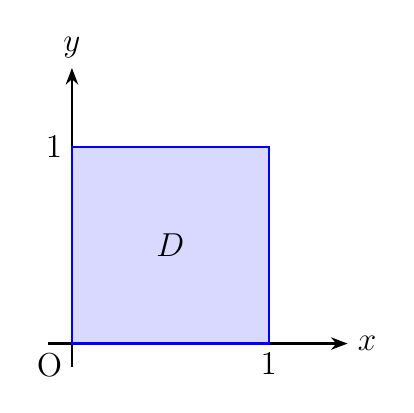
\begin{tikzpicture}[every node/.style={font=\large}]
  % Axes
  \draw[-{Stealth[length=6pt]}, thick] (-0.3,0) -- (3.5,0) node[right] {$x$};
  \draw[-{Stealth[length=6pt]}, thick] (0,-0.3) -- (0,3.5) node[above] {$y$};

  % Shaded square region
  \fill[blue!15] (0,0) rectangle (2.5,2.5);
  \draw[thick, blue] (0,0) rectangle (2.5,2.5);

  % Labels
  \node[below] at (2.5,0) {$1$};
  \node[left] at (0,2.5) {$1$};
  \node at (1.25,1.25) {$D$};

  % Origin
  \node[below left] at (0,0) {O};
\end{tikzpicture}
\end{document}
